\documentclass[xcolor=svgnames,17pt]{beamer}

\usepackage[export]{adjustbox}
\usepackage{bookmark}
\usepackage{colortbl} \arrayrulecolor[gray]{0.7}
\usepackage{microtype}
\usepackage{pgfpages}
\usepackage{rotating}
\usepackage{textcomp}
\usepackage{tabularx}
\usepackage{xspace}

\usepackage{fontspec}

\hypersetup{hidelinks,pdfpagemode=}

\urlstyle{same}

\newcommand*{\sizefont}[1]{%
    \ifcase#1\relax
    \or \tiny
    \or \scriptsize
    \or \footnotesize
    \or \small
    \or \normalsize
    \or \large
    \or \Large
    \or \LARGE
    \or \huge
    \or \Huge
    \fi}

%%

\newcommand*{\mybullet}{\tikz[baseline=-.6ex]\node[%
    draw,circle,inner sep = -0.15ex,fill]{.};\xspace}

\setbeamertemplate{footline}{
    \usebeamercolor[fg]{page number in head/foot}%
    \usebeamerfont{page number in head/foot}%
    \hspace*{1ex}\insertframenumber\,/\,\inserttotalframenumber\hfill
    github.com/andrewdotn/vixpy\ }

\newcommand*{\plainfooter}{%
    \setbeamertemplate{footline}{
        \usebeamercolor[fg]{page number in head/foot}%
        \usebeamerfont{page number in head/foot}%
        \hspace*{1ex}\insertframenumber\,/\,\inserttotalframenumber\vskip2pt}}

\makeatletter
\def\alphslide{\@alph{\intcalcAdd{1}{\intcalcSub{\thepage}{\beamer@framestartpage}}}}
\newcommand*{\plainstepfooter}{
    \setbeamertemplate{footline}{
        \usebeamercolor[fg]{page number in head/foot}%
        \usebeamerfont{page number in head/foot}%
        \hspace*{1ex}\insertframenumber\alphslide\,/\,\inserttotalframenumber\vskip2pt}}
\makeatother

\setbeamertemplate{note page}{
    \sizefont{3}
    \setlength{\parskip}{10pt}
    \insertnote
    \par}

\setbeamertemplate{navigation symbols}{}
\setbeamerfont{title}{size=\LARGE}
\setbeamerfont{frametitle}{size=\LARGE}
\setbeamerfont{framesubtitle}{size=\normalsize}

\newcommand*{\tocsection}[1]{\pdfbookmark[2]{#1}{#1}}

%%

\title{Driving VMware with Python: vixpy}

\author{\texorpdfstring{%
    Andrew Neitsch}{Andrew Neitsch}}

\date{\small 2015-11-27}

\begin{document}

\tocsection{Title page}

\begin{frame}[plain]
\titlepage
\adjustbox{width=0.9\paperwidth,center}{\structure{\href{https://github.com/andrewdotn/vixpy}{github.com/andrewdotn/vixpy}}}
\end{frame}

\begin{frame}{Outline}
\tableofcontents
\end{frame}

\section{Motivation}

\begin{frame}{Testing services}

\begin{itemize}
\item Unit tests are great for individual modules of code
\pause
\item End-to-end testing requires deploying the code \ldots
\pause\ to multiple machines \ldots
\pause
\item setting up prerequisites like databases \ldots
\pause
\item and configuration management \ldots
\pause
\item and sometimes with specialized networking needs too.
\end{itemize}

\end{frame}

\begin{frame}{Example: OpenVPN}
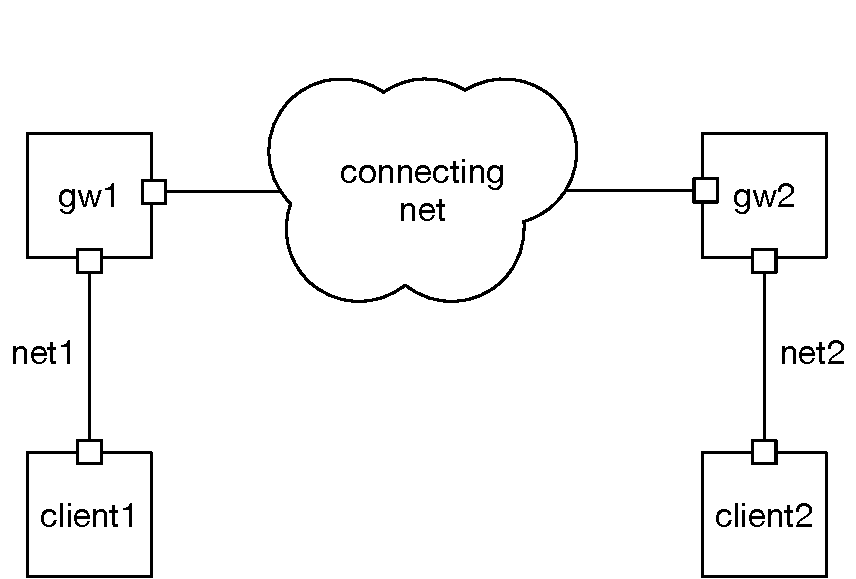
\includegraphics[max width=0.9\paperwidth,center,page=1]{OpenVPN.pdf}
\end{frame}

\begin{frame}{Example: OpenVPN}
\includegraphics[max width=0.9\paperwidth,center,page=2]{OpenVPN.pdf}
\end{frame}

\begin{frame}{Example: OpenVPN}
\includegraphics[max width=0.9\paperwidth,center,page=3]{OpenVPN.pdf}
\end{frame}

\begin{frame}{Example: OpenVPN}
\includegraphics[max width=0.9\paperwidth,center,page=4]{OpenVPN.pdf}
\end{frame}

\begin{frame}{Example: OpenVPN}
\includegraphics[max width=0.9\paperwidth,center,page=5]{OpenVPN.pdf}
\end{frame}

\begin{frame}{Example: OpenVPN}
\includegraphics[max width=0.9\paperwidth,center,page=6]{OpenVPN.pdf}
\end{frame}

\begin{frame}{Example: OpenVPN}
\centering
Testing this requires at least 4 VMs \\
and three networks
\end{frame}

\begin{frame}[fragile]{Typical solution: Vagrant}

\small

Vagrantfile:

{
\leftskip=1in
\begin{verbatim}
Vagrant.configure(2) do |config|
  config.vm.box = "bento/centos-7.1"

  %w[client1 gw1 gw2 client2 cm].each do |name|
    config.vm.define name
  end
end
\end{verbatim}
}

\texttt{\$ vagrant up \\ ...}
\end{frame}

\begin{frame}{Typical solution: Vagrant}
Advantages:
\begin{itemize}
\item declarative specification file
\item \texttt{vagrant} command-line tool
\item support for 20+ cloud providers
\end{itemize}
\end{frame}

\begin{frame}{Typical solution: Vagrant}
Disadvantages for automatic service testing:
\begin{itemize}
\item declarative specification file
\only<2>{
    \begin{itemize}
    \item Tricky to configure dynamically
    \end{itemize}
}
\item \texttt{vagrant} command-line tool
\only<3>{
    \begin{itemize}
    \item no API for interacting with VMs
    \end{itemize}
}
\item support for 20+ cloud providers
\only<4>{
    \begin{itemize}
    \item lowest-common-denominator support
    \item no snapshots
    \item no cloning
    \end{itemize}
}
\end{itemize}
\end{frame}

\begin{frame}{Typical solution: vagrant}
\begin{itemize}
\item really, really slow
\item making a mistake means starting over
\item can’t actually test OpenVPN due to networking issues
\end{itemize}
\end{frame}

\begin{frame}{VMware Fusion/Workstation}
\begin{itemize}
\item Really fast
\item Linked clones
\item Snapshots
\end{itemize}
\pause
Can we drive it programatically to get something faster and easier to use?
\end{frame}

\begin{frame}{vmrun}

VMware Fusion.app/Contents/Library/vmrun \\[0.25in]

\sizefont 2
\texttt{%
start stop reset suspend pause unpause listSnapshots snapshot
deleteSnapshot revertToSnapshot runProgramInGuest fileExistsInGuest
directoryExistsInGuest setSharedFolderState addSharedFolder
removeSharedFolder enableSharedFolders disableSharedFolders
listProcessesInGuest killProcessInGuest runScriptInGuest deleteFileInGuest
createDirectoryInGuest deleteDirectoryInGuest listDirectoryInGuest
renameFileInGuest captureScreen writeVariable readVariable
getGuestIPAddress list upgradevm installTools checkToolsState
deleteVM clone
}

\end{frame}

\begin{frame}[fragile]{VIX}

\texttt{VMware Fusion.app/Contents/Public} \\
\centering{\texttt{vix.h} and shared library}

\small
\structure{\href{https://www.vmware.com/support/developer/vix-api/}{%
    vmware.com/support/developer/vix-api}}

\sizefont 2
\begin{verbatim}
jobHandle = VixVM_PowerOn(vmHandle,
                          VMPOWEROPTIONS,
                          VIX_INVALID_HANDLE,
                          NULL, // *callbackProc,
                          NULL); // *clientData);
err = VixJob_Wait(jobHandle, VIX_PROPERTY_NONE);
if (VIX_FAILED(err)) {
    printf("PowerOn failed\n");
    goto fail;
}
\end{verbatim}

\end{frame}

\section{Getting it working}

\begin{frame}{}
\tableofcontents[currentsection]
\end{frame}

\begin{frame}{Cython}

\begin{itemize}
\item Python code gets compiled into a Python C module
\item Can do whatever C or Python can do
\item Didn’t have to read the manual
\item Though there is an O’Reilly book
\end{itemize}

\end{frame}

\begin{frame}[fragile]{Example: Python to C}

\begin{verbatim}
def hi(x):
    return x + 42
\end{verbatim}

\end{frame}

\begin{frame}[fragile]{Python to C and back}

\sizefont 2
\begin{verbatim}
$ cython foo.pyx
$ wc -l foo.c
1737
$ cat foo.c
...
/* "foo.pyx":2
 * def hi(x):
 *     return x + 42             # <<<<<<<<<<<<<<
 */
  __Pyx_XDECREF(__pyx_r);
  __pyx_t_1 = __Pyx_PyInt_AddObjC(__pyx_v_x, __pyx_int_42, 42, 0); if (unlikely(!__pyx_t_1)) {__pyx_filename = __pyx_f[0]; __pyx_lineno = 2; __pyx_clineno = __LINE__; goto __pyx_L1_error;}
  __Pyx_GOTREF(__pyx_t_1);
...
$ gcc -shared foo.c -o foo.so -lpython \
    -I/System/Library/Frameworks/Python.framework/Headers
$ python -c 'import foo; print foo.hi(42)'
84
\end{verbatim}

\end{frame}

\begin{frame}[fragile]{Example: C to Python}
\sizefont 3
\begin{verbatim}
$ cat foo.pyx
cdef extern:
    int printf(const char* s, ...)

def blah(x):
    printf("hi there, x is at %p\n", <void*>x)
$ cython ... && gcc ...
$ python -c 'import foo; foo.blah(42)'
hi there, x is at 0x7fe183605be8
\end{verbatim}

\pause
\normalsize

cdefs aren’t exported, idea seems to be to use them to create a pythonic
interface
\end{frame}

\begin{frame}{Cython for VIX}
\adjustbox{width=0.7\paperwidth,center}{It just worked!} \\
\pause
\centering
\vspace*{1.5\baselineskip}
\href{https://github.com/andrewdotn/vixpy}{\structure{the code}}
\end{frame}

\begin{frame}{Cython for VIX}
Time to
\begin{itemize}
\item clone a VM
\item run a command
\item delete the VM
\end{itemize}

\vspace\baselineskip

\begin{tabular}{lr}
vagrant & 69 seconds \\
\pause
vixpy & 10 seconds
\end{tabular}

\end{frame}

\section{Parallelizing it}

\begin{frame}{}
\tableofcontents[currentsection]
\end{frame}

\begin{frame}{VixJob\_Wait()}

called with Python interpreter lock held

\vspace\baselineskip

no point in spawning other threads—\\
they’ll just block

\end{frame}

\setlength\fboxsep{1pt}
\def\h#1{\colorbox{yellow}{#1}}

\small
\begin{frame}{Async callbacks}
\texttt{%
VixVM\_PowerOn(vmHandle, \\
\ \ \ \ \ \ \ \ \ \ \ \ \ \ VMPOWEROPTIONS, \\
\ \ \ \ \ \ \ \ \ \ \ \ \ \ VIX\_INVALID\_HANDLE, \\
\ \ \ \ \ \ \ \ \ \ \ \ \ \ \h{NULL, // *callbackProc} \\
\ \ \ \ \ \ \ \ \ \ \ \ \ \ \h{NULL); // *clientData}
}

\vspace\baselineskip

\href{https://github.com/cython/cython/tree/master/Demos/callback/cheese.pyx}{%
    \structure{cython Demos/callback/cheese.pyx}}

\end{frame}

\begin{frame}{Async callback trouble}

\sizefont{3}
\texttt{%
78304 Segmentation fault: 11\ \ python test.py \\
make: *** [all] Error 139 \\
... \\
\pause
lldb> expr *\_\_pyx\_t\_1->ob\_type \\
... \\
\pause
CFLAGS=-g ./configure \&\& make \\
... \\
\pause
Fatal Python error: take\_gil: NULL tstate
}

\end{frame}

\begin{frame}[fragile]{Eventually found \texttt{nogil}}

\begin{verbatim}
cdef VixJob_Wait() nogil
...
with nogil:
    retCode = VixJob_Wait(...)
\end{verbatim}

If you’re careful not to use Python objects— \\[0.5\baselineskip]
Enables standard threads to run concurrently!

\end{frame}

\section{Results}

\begin{frame}{Results}

Time to clone five test VMs, run a command in each, and then destroy them:

\pause
\vspace*{1.5\baselineskip}

\centering
\begin{tabular}{lr}
vagrant\ \ \  & 5 minutes 45 seconds \\
\pause
vixpy & 16 seconds
\end{tabular}
\vspace*{1.5\baselineskip}

\pause

\textasciitilde20x faster

\end{frame}

\section{Conclusions}

\begin{frame}{Conclusions}
Cython is fantastic
\begin{itemize}
\item For calling C libraries
\item For rewriting hot spots in C
\end{itemize}
\pause
VIX is promising\pause{}—future work:
\begin{itemize}
\item Clean up snapshots
\pause
\item Allow showing GUI
\pause
\item Flesh out APi
\pause
\item Iterate on my OpenVPN setup
\end{itemize}
\end{frame}

\begin{frame}
\adjustbox{width=0.5\paperwidth,center}{\structure{Questions?}}
\end{frame}

\begin{frame}{Call for talks}

“w/o interesting talks, there's not a ton of point in ‘meeting up’”

\pause

\begin{enumerate}
\item Pick something you find interesting
\item Talk about it
\item Include suggestions for stuff to hack on
\end{enumerate}

\end{frame}

\begin{frame}{Suggested exercises}
\begin{itemize}
\item Get the code running on your machine
\item Use Cython to call a useful C library
\item Use vixpy to launch a multi-tier application
\end{itemize}
\end{frame}

\end{document}
